% This is samplepaper.tex, a sample chapter demonstrating the
% LLNCS macro package for Springer Computer Science proceedings;
% Version 2.21 of 2022/01/12
%
\documentclass[runningheads]{llncs}
%
\usepackage{algorithm}
\usepackage{algorithmic}
\usepackage{subcaption}
\usepackage[T1]{fontenc}
\usepackage{amsmath}
% T1 fonts will be used to generate the final print and online PDFs,
% so please use T1 fonts in your manuscript whenever possible.
% Other font encondings may result in incorrect characters.
%
\usepackage{graphicx}
% Used for displaying a sample figure. If possible, figure files should
% be included in EPS format.
%
% If you use the hyperref package, please uncomment the following two lines
% to display URLs in blue roman font according to Springer's eBook style:
%\usepackage{color}
%\renewcommand\UrlFont{\color{blue}\rmfamily}
%\urlstyle{rm}
%
\begin{document}
%
\title{Edge-Critical Strongly Connected Directed Graphs}
%
%\titlerunning{Abbreviated paper title}
% If the paper title is too long for the running head, you can set
% an abbreviated paper title here
%
\author{Abhinav Kumar Verma\inst{1} \and
Akrati Saxena\inst{2}\orcidID{0000-0002-7151-6309}}
%
\authorrunning{A. K. Verma and A. Saxena}
% First names are abbreviated in the running head.
% If there are more than two authors, 'et al.' is used.
%
\institute{Department of Electronics and Electrical Communications, Indian Institute of Technology, Kharagpur, India 
\and
The Leiden Institute of Advanced Computer Science, Universiteit Leiden, the Netherlands
\email{a.saxena@liacs.leidenuniv.nl}\\
}
%
\maketitle              % typeset the header of the contribution
%
\begin{abstract}
We propose an iterative algorithm for generation of all edge-critical strongly connected directed graphs. A proof of correctness of the algorithm is also provided.

\keywords{edge-criticality \and strongly connected \and directed graph \and spanning tree.}
\end{abstract}
%
%
%
\section{Introduction}
A directed graph is strongly connected if there exists a path between any pair of nodes. It is edge-critical, if the strongly connected digraph ceases to be strongly connected when any of its edge is removed. The Tarjan algorithm is used to test the strong connectivity of a digraph. The algorithm determines strong connectedness in $\mathcal{O}(|E|)$. Assuming self loops and multiple edges are not allowed, there exists only one digraph of two nodes that is strongly connected. Coincidentally, it is edge-critical too.


\subsubsection{Our Contributions.} We propose an algorithm to test the edge criticality of a strongly connected digraph in $\mathcal{O}(|E|^2)$. Then, we propose an iterative algorithm to construct a set of all unlabelled edge-critical strongly connected directed graphs with N+1 nodes provided a set of all such graphs with N nodes. The edge-criticality of the graphs constructed by the algorithm is self-evident. We provide a proof for the completeness of the algorithm i.e. all edge-critical strongly connected digraphs of N+1 nodes are constructed by the algorithm.

\section{Algorithms}

\subsection{Edge-Criticality of a Strongly Connected Digraph}
% To develop the algortihm for construction of all edge-critical strongly connected digraphs, we first need an algorithm to test the edge-criticality of a strongly connected digraph. The psuedocode and explanation of this algorithm is provided below. Note that it is a trivial extension of the Tarjan algorithm.

\begin{algorithm}
\caption{Test Edge-Criticality}
\label{alg:edge_criticality}
\begin{algorithmic}[1]
\REQUIRE A strongly connected directed graph $G = (V, E)$
\ENSURE Whether $G$ is edge-critical
\FOR{each edge $e \in E$}
    \STATE Remove edge $e$ from $G$ to create $G'$
    \STATE Test if $G'$ is strongly connected using Tarjan's algorithm
    \IF{$G'$ is not strongly connected}
        \STATE Restore edge $e$ in $G$
    \ELSE
        \RETURN $G$ is not edge-critical
    \ENDIF
\ENDFOR
\RETURN $G$ is edge-critical
\end{algorithmic}
\end{algorithm}
 
 To test if a strongly connected digraph is edge-critical, Tarjan algorithm is employed repetitively with removal of an edge with replacement from the digraph. If the edge-removed digraph remains strongly connected, then the original digraph is not edge-critical. A pseudo-code for this algorithm is provided below.

\subsection{Construction of All N+1 Nodes Edge-Critical Strongly Connected Digraphs}
% Now we propose the main algorithm for the construction of all edge-critical strongly connected digraphs of N+1 nodes from a set of all such graphs of N nodes. 

\begin{algorithm}
\caption{Construct Edge-Critical Strongly Connected Digraphs}
\begin{algorithmic}[1]
\REQUIRE Set of edge-critical strongly connected digraphs $\mathcal{P}_N$ with $N$ nodes
\ENSURE Set $\mathcal{Q}$ of edge-critical strongly connected digraphs with $N+1$ nodes
\STATE Initialize empty set $\mathcal{Q}$
\FOR{each digraph $\mathcal{G} \in \mathcal{P}_N$}
    \STATE Construct set $\mathcal{L} = \text{Nodes}(\mathcal{G}) \times \text{Nodes}(\mathcal{G})$
    \FOR{each pair $(a, b) \in \mathcal{L}$}
        \STATE Initialize $\mathcal{G}_{(a, b)}$ = $\mathcal{G}$
        \STATE Add unconnected node $\mathcal{V}_{\text{new}}$ to $\mathcal{G}_{(a, b)}$
        \STATE Add edges $(a, \mathcal{V}_{\text{new}})$ and $(\mathcal{V}_{\text{new}}, b)$  to $\mathcal{G}_{(a, b)}$
        \IF{$(a, b) \in \text{Edge}(\mathcal{G})$}
            \STATE Remove edge $(a, b)$ from $\mathcal{G}_{(a, b)}$
        \ELSE
            \IF{graph $\mathcal{G}_{(a, b)}$ is not edge-critical}
                \STATE \textbf{continue}
            \ENDIF
        \ENDIF
        \IF{$\mathcal{G}_{(a, b)}$ and its isomorphs $\notin \mathcal{Q}$}
            \STATE Add $\mathcal{G}_{(a, b)}$ to $\mathcal{Q}$
        \ENDIF
    \ENDFOR
\ENDFOR
\RETURN $\mathcal{Q}$
\end{algorithmic}
\end{algorithm}

Let us denote the set of all edge-critical strongly connected digraphs with N nodes as $\mathcal{P}_N$. We initiate an empty set $\mathcal{Q}$ to store the constructed digraphs with N+1 nodes. A digraph $\mathcal{G}$ is popped from $\mathcal{P}_N$ and an unconnected node $\mathcal{V}_{new}$ is added to the digraph. A set $\mathcal{L = }Nodes({G}) {\times} Nodes ({G})$ of all possible pairs of nodes is constructed. 

Iteratively, a pair (a, b) is popped from the set $\mathcal{L}$. If $\mathcal (a,b) \in Edge({G})$, then the edge (a,b) is removed and edges (a, $\mathcal{V}_{new}$) and ($\mathcal{V}_{new}$, b) are added to construct $\mathcal{G}_{(a, b)}$, an edge-critical strongly connected digraph of N+1 edges. If this graph and its isomorphs are not a member of $\mathcal{Q}$, then the graph is added to the set $\mathcal{Q}$.

If $\mathcal (a,b) \notin Edge({G})$, then the edges (a, $\mathcal{V}_{new}$) and ($\mathcal{V}_{new}$, b) are added and the resulting graph is checked for edge-criticality. If this graph is edge-critical and neither the graph nor its isomorphs are a member of $\mathcal{Q}$, then the graph is added to the set $\mathcal{Q}$. A pseudo-code for this algorithm is provided below.


% Then in your document:
\begin{figure}[htbp]
    \centering
    \begin{subfigure}{0.48\textwidth}
        \centering 
        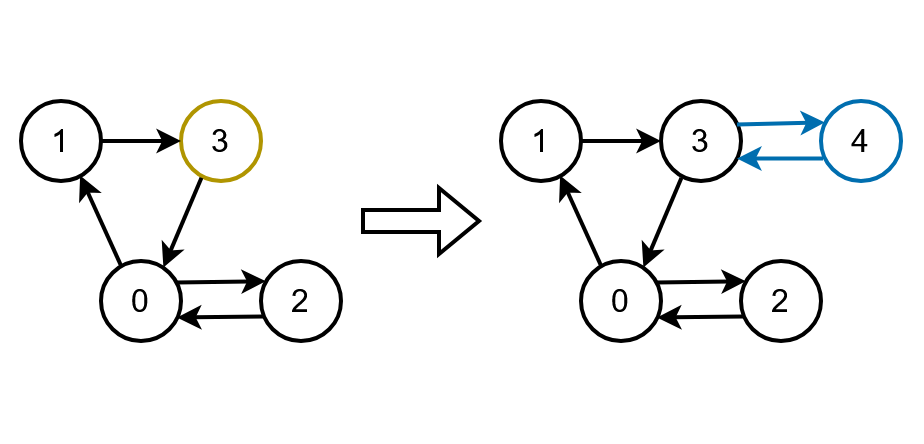
\includegraphics[width=\textwidth]{fig1_a.png}
        \caption{a = 2, b = 0, and (2, 0) $\in \text{Edge}(\mathcal{G})$. When (a, b) $\in \text{Edge}(\mathcal{G})$, the extended digraph is always edge-critical.}
        \label{fig:1a}
    \end{subfigure}
    \hfill
    \begin{subfigure}{0.48\textwidth}
        \centering
        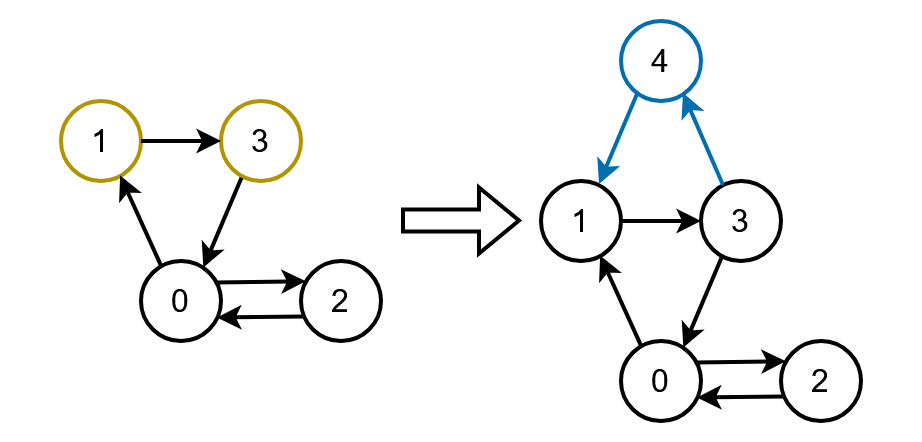
\includegraphics[width=\textwidth]{fig1_b.png}
        \caption{a = 3, b = 1, and (3, 1) $\notin \text{Edge}(\mathcal{G})$. Constructed digraph $\mathcal{G}_{(3, 1)}$ is edge-critical.}
        \label{fig:1b}
    \end{subfigure}
    
    \vspace{10pt}
    
    \begin{subfigure}{0.48\textwidth}
        \centering
        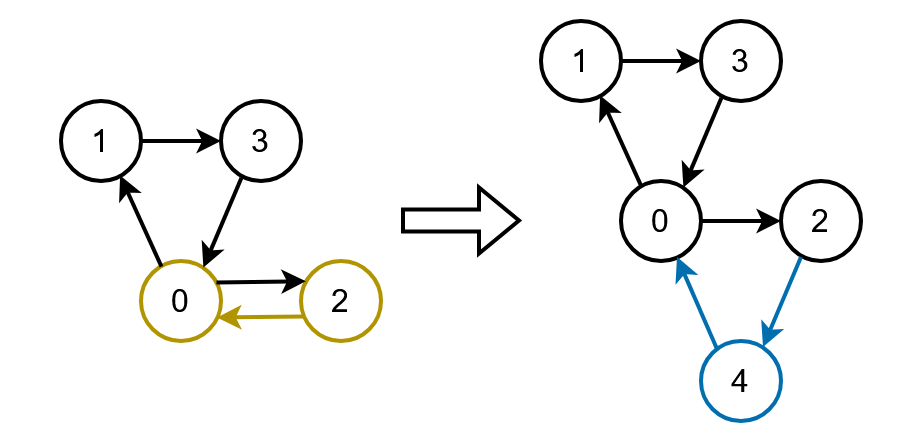
\includegraphics[width=\textwidth]{fig1_c.png}
        \caption{a = 3, b = 3, and (3, 3) $\notin \text{Edge}(\mathcal{G})$. Constructed digraph $\mathcal{G}_{(3, 3)}$ is edge-critical.}
        \label{fig:1c}
    \end{subfigure}
    \hfill
    \begin{subfigure}{0.48\textwidth}
        \centering
        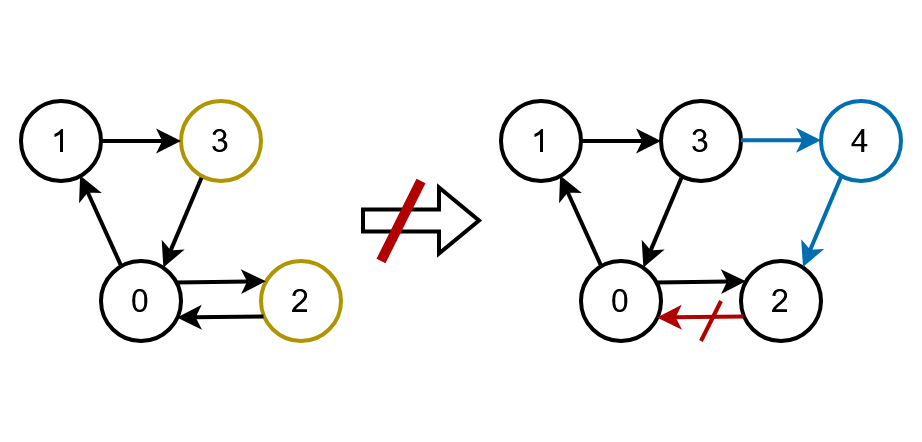
\includegraphics[width=\textwidth]{fig1_d.png}
        \caption{a = 3, b = 2, and (3, 2) $\notin \text{Edge}(\mathcal{G})$. Constructed digraph $\mathcal{G}_{(a, b)}$ is not edge-critical, thus it is not added to the set $\mathcal{Q}$.}
        \label{fig:1d}
    \end{subfigure}
    \caption{Extension of an edge-critical strongly connected digraph of 4 nodes to 5 node digraph by the algorithm. Nodes of the existitng digraph are numbered from 0 to 3 and $\mathcal{V}_{\text{new}}$ = 4 for all four cases. Yellow highlights indicate nodes and edges affected during the extension process, while blue highlights show both newly added edges and the nodes involved in these new connections. The red edge with a stroke is redundant and its removal doesn't affect strong connectedness of digraph.}
    \label{fig:complete}
\end{figure}

\section{Proofs}

\subsection{Edge-Criticality Algorithm}
The correctness of edge-criticality algorithm can be directly verified using the definition of an edge-critical digraph. A strongly connected digraph is not edge-critical if it maintains strong connectivity after the removal of any single edge. Conversely, if the removal of any edge destroys the strong connectivity of the digraph, then the digraph is edge-critical. The algorithm directly leads to this definition.

\subsection{Correctness of the Construction Algorithm}
In this section, we prove that any digraph in the set $\mathcal{Q}$ is necessarily edge-critical strongly connected digraph. We proceed by proving two theorems that correspond to  the scenarios, $(a, b) \notin \text{Edge}(\mathcal{G})$ and $(a, b) \in \text{Edge}(\mathcal{G})$. 

\vspace{0.5em}
\noindent We use these notations and description of a digraph $\mathcal{G}_{(a,b)}$ for the following theorems and the proofs.

\begin{align*}
    &\mathcal{V} = Nodes(\mathcal{G}); \\
    &e_{in} = edge (a, \mathcal{V}_{\text{new}}); \\
    &e_{out} = edge (\mathcal{V}_{\text{new}}, b); \\
    &Nodes(\mathcal{G}_{(a,b)}) = \mathcal{V} \cup \mathcal{V}_{\text{new}} = \mathcal{W}; \\
    &Edges(\mathcal{G}_{(a,b)}) = Edges(\mathcal{G}) \cup e_{in} \cup e_{out}; \\
\end{align*}

\begin{theorem}
If $\mathcal{G}$ is an edge-critical strongly connected digraph with nodes a and b such that (a, b) $\notin$ Edges($\mathcal{G}$) then the graph $\mathcal{G}_{(a,b)}$ is a strongly connected digraph.
\end{theorem}

\begin{proof}
We observe that there exists a path from any node in set $\mathcal{V}$ to any other node in the same set because the original graph $\mathcal{G}$ is strongly connected. $a \in \mathcal{V}$, $b \in \mathcal{V}$, and there exists a path from $\mathcal{V}_{\text{new}}$ to the node $b$ and from the node $a$ to node $\mathcal{V}_{\text{new}}$. Thus, there must exist a path from $\mathcal{V}_{\text{new}}$ to any node in $\mathcal{V}$, from any node in $\mathcal{V}$ to $\mathcal{V}_{\text{new}}$, and from $\mathcal{V}_{\text{new}}$ to $\mathcal{V}_{\text{new}}$. So, there exists a path from any node in $\mathcal{W}$ to any other node in the same set. Hence, $\mathcal{G}_{(a,b)}$ is strongly connected.
\end{proof}

\begin{figure}[ht]
    \centering
    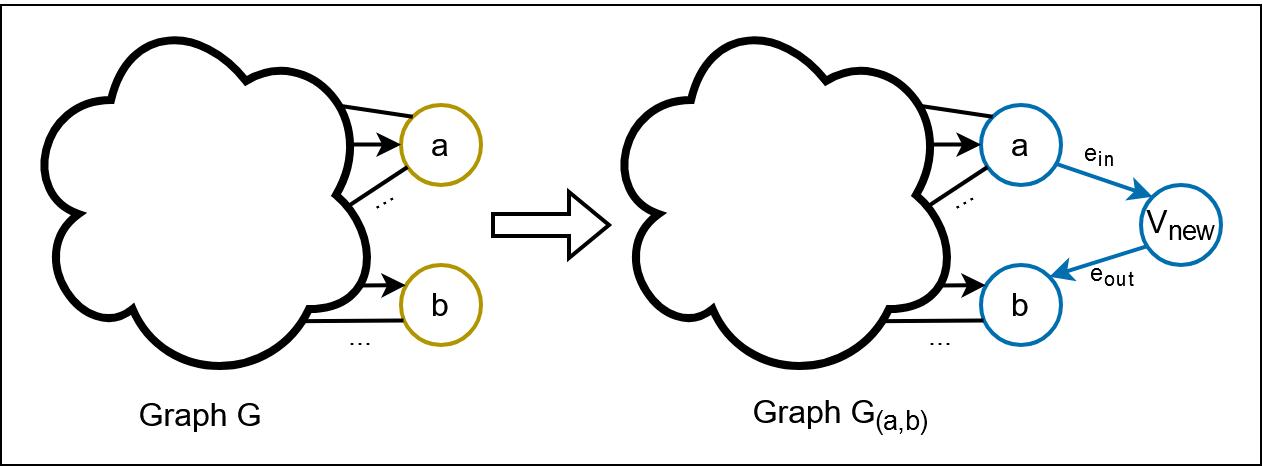
\includegraphics[width=0.7\textwidth]{fig2.png}
    \caption{Transformation of a edge-critical strongly connected digraph $\mathcal{G}$ to a strongly connected digraph $\mathcal{G}_{(a,b)}$ when (a, b) $\notin$ Edges($\mathcal{G}$).}
    \label{fig:fig2}
\end{figure}

\noindent\textbf{Note:} The digraph $\mathcal{G}_{(a,b)}$ is not necessarily edge-critical and therefore we require to check the edge-criticality explicitly in the algorithm for $(a, b) \notin \text{Edges}(\mathcal{G})$ scenario.

\vspace{0.5em}
\noindent In addition we use these notations and description of a digraph $\mathcal{G'}_{(a,b)}$ for the next theorem and its proof.
\begin{align*}
    &e_{-} = edge (a, b); \\
    &Nodes(\mathcal{G'}_{(a,b)}) = Nodes(\mathcal{G}_{(a,b)}); \\
    &Edges(\mathcal{G'}_{(a,b)}) = Edges(\mathcal{G}_{(a,b)}) \setminus e_{-}.
\end{align*}

\begin{theorem}
If $\mathcal{G}$ is an edge-critical strongly connected digraph with nodes a and b such that (a, b) $\in$ Edges($\mathcal{G}$) then the graph $\mathcal{G'}_{(a,b)}$ is also an edge-critical strongly connected digraph.
\end{theorem}

In this scenario, the edge $e_{-} = (a, b)$ is replaced by two edges $e_{in}$ and $e_{out}$ preserving the connectivity from node a to b. 

\begin{proof}
As the original graph $\mathcal{G}$ was strongly connected, there must exist a path from any node in $\mathcal{V}$ to any other node in the same set on graph $\mathcal{G'}_{(a, b)}$. If the path contained edge $e_{-}$ on $\mathcal{G}$ then it would instead contain $e_{in}$ and $e_{out}$ on $\mathcal{G}_{(a, b)}$. Also there exists a path from from $\mathcal{V}_{\text{new}}$ to the node b and from the node a to node $\mathcal{V}_{\text{new}}$, so there must exist a path from $\mathcal{V}_{\text{new}}$ to any node in $\mathcal{V}$ and from any node in $\mathcal{V}$ to $\mathcal{V}_{\text{new}}$. Furthermore, the path $e_{out} \cup Path(b, a) \cup e_{in}$ connects $\mathcal{V}_{\text{new}}$ to itself. So, there exists a path from any node in $\mathcal{W}$ to another node in the set. Hence, $\mathcal{G'}_{(a, b)}$ is strongly connected.

If the edge $e_{in}$ is removed, then there doesn't exist any path from the node a to node $\mathcal{V}_{\text{new}}$. Similarly, if the edge $e_{out}$ is removed, then there doesn't exist any path from the node $\mathcal{V}_{\text{new}}$ to node b. Thus with removal of either of these edges, the graph $\mathcal{G'}_{(a, b)}$ ceases to be strongly connected. 

The graph $\mathcal{G}$ was edge-critical. If any edge $e = (x, y) \neq e_{-}$ is removed from the graph $\mathcal{G}$, then there exists no path from the node x to the node y on the graph $\mathcal{G}$. This must be the case otherwise the edge $e$ would be redundant. Now consider the edge $e$ on the new graph $\mathcal{G'}_{(a, b)}$. Here too, if the edge $e$ is removed, there must not exist any path from the node $x$ to the node $y$ because if such a path existed on $\mathcal{G'}_{(a, b)}$, then the path would exist on $\mathcal{G}$ too with possible replacement of $\{e_{in}\} \cup \{e_{out}\}$ by $\{e_{-}\}$. Thus removal of any edge from the graph $\mathcal{G'}_{(a, b)}$, dissolves its strong connectedness. Hence, $\mathcal{G'}_{(a, b)}$ is edge-critical strongly connected digraph.
\end{proof}

\begin{figure}[ht]
    \centering
    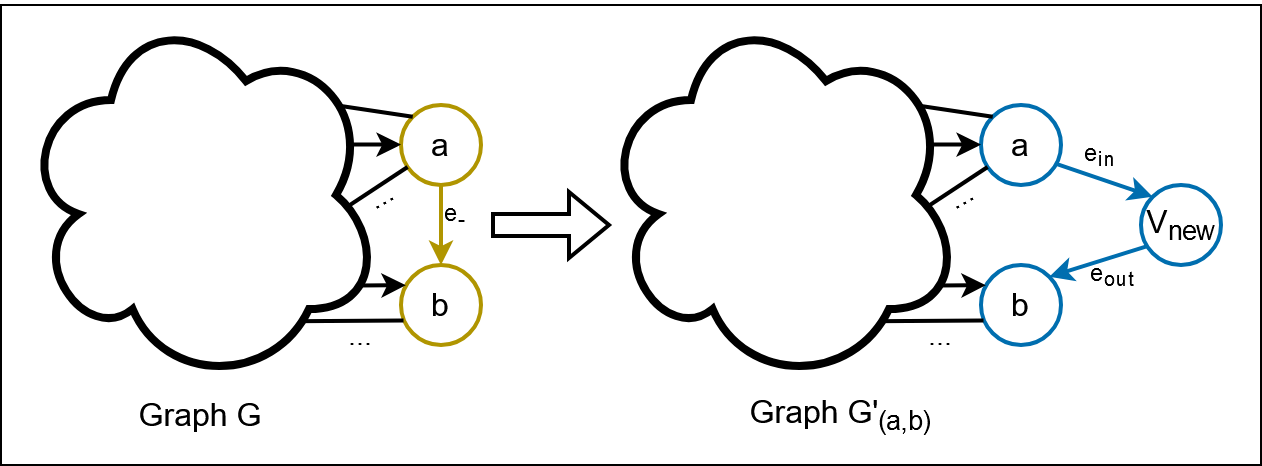
\includegraphics[width=0.7\textwidth]{fig3.png}
    \caption{Transformation of a edge-critical strongly connected digraph $\mathcal{G}$ to another edge-critical strongly connected digraph $\mathcal{G'}_{(a,b)}$ when (a, b) $\in$ Edges($\mathcal{G}$).}
    \label{fig:fig3}
\end{figure}

\noindent With these theorems, the correctness of algorithm is established i.e. each element of the output set $\mathcal{Q}$ is edge-critical strongly connected digraph. Now, we proceed to prove the completeness of the algorithm i.e. the set $\mathcal{Q}$ contains all possible edge-critical strongly connected digraph of N+1 nodes, if it receives a set of all possible edge-critical strongly connected digraph of N ndoes as its input.

\subsection{Reduction of Edge-Critical Strongly Connected Digraphs to Smaller Node Counts}
% Reduction of an edge-critical strongly connected digraph with N+1 nodes and a node of degree 2 to an edge-critical strongly connected digraph with N nodes.

% For the following theorem and its proof, we assume $\mathcal{G}$ to be an edge-critical strongly connected graph with a node $V_{red}$ having one in-edge $e_{in}$ and one out-edge $e_{out}$ only. The node $a$ is pre-node of $e_{in}$ and the node $b$ is the post-node of $e_{out}$.
\begin{theorem}
If an edge-critical strongly connected digraph $\mathcal{G}$ has a node $V_{red}$ with one in-edge ($e_{in}$) and one out-edge ($e_{out}$) only, then the digraph can be reduced to another edge-critical strongly connected digraph with one fewer node by performing one of the following operations:
\begin{enumerate}
    \item Removing the node $V_{red}$ and the edges $e_{in}$ and $e_{out}$; or
    \item Removing the node $V_{red}$, removing the edges $e_{in}$ and $e_{out}$, and adding an edge from the pre-node of $e_{in}$ to the post-node of $e_{out}$.
\end{enumerate}
\end{theorem}

\begin{proof}
Let us assume that the pre-node of $e_{in}$ is $a$ and the post-node of $e_{out}$ is $b$ on the graph $\mathcal{G}$. Now, we construct a graph $\mathcal{H}$ from the graph $\mathcal{G}$ by following the second operation i.e. removing the node $V_{red}$, removing the edges $e_{in}$ and $e_{out}$, and adding an edge $e = (a, b)$. Now let $\mathcal{V} = Nodes(\mathcal{G})$ and $\mathcal{W} = Nodes(\mathcal{H})$.

The digraph $\mathcal{G}$ is strongly connected so it is possible to reach from any node in the set $\mathcal{V}$ to another node in the set on $\mathcal{G}$. Since $\mathcal{W} \subset \mathcal{V}$, a path exists from any node in $\mathcal{W}$ to another node in the set on the graph $\mathcal{H}$ with the possibility of including the edge $\{e\}$ in the path instead of $\{e_{in}\} \cup \{e_{out}\}$, if the latter is a component of the path on the graph $\mathcal{G}$. Thus, the graph $\mathcal{H}$ is strongly connected.

The graph $\mathcal{G}$ is edge-critical. If any edge $e = (x, y)$ other than $e_{in}$ and $e_{out}$ is removed from the graph $\mathcal{G}$, then there exists no path from the node x to the node y on the graph $\mathcal{G}$. Now consider the edge $e$ on the graph $\mathcal{H}$. Here too, if the edge $e$ is removed, there must not exist any path from the node $x$ to the node $y$ because if such a path existed on $\mathcal{H}$, then the path would exist on $\mathcal{G}$ too with possible replacement of $\{e_{in}\} \cup \{e_{out}\}$ by $\{e\}$. Thus removal of any edge from the graph $\mathcal{H}$ except possibly $(a, b)$, dissolves its strong connectedness.

Now, we construct a graph $\mathcal{H'}$ by removing the edge {e} from the graph $\mathcal{H}$. This construction corresponds to the first operation. If the graph $\mathcal{H'}$ is strongly connected then it is also edge-critical following the above-mentioned argument. However, if it is not strongly connected, then $\mathcal{H}$ is necessarily edge-critical as removal of any of its edge including edge $e$ dissolves the strong connectedness of the graph. Hence, either the graph $\mathcal{H'}$ composed by first operation or the graph $\mathcal{H}$ composed by second operation must be an edge-critical strongly connected digraph.
\end{proof}

\begin{figure}[ht]
    \centering
    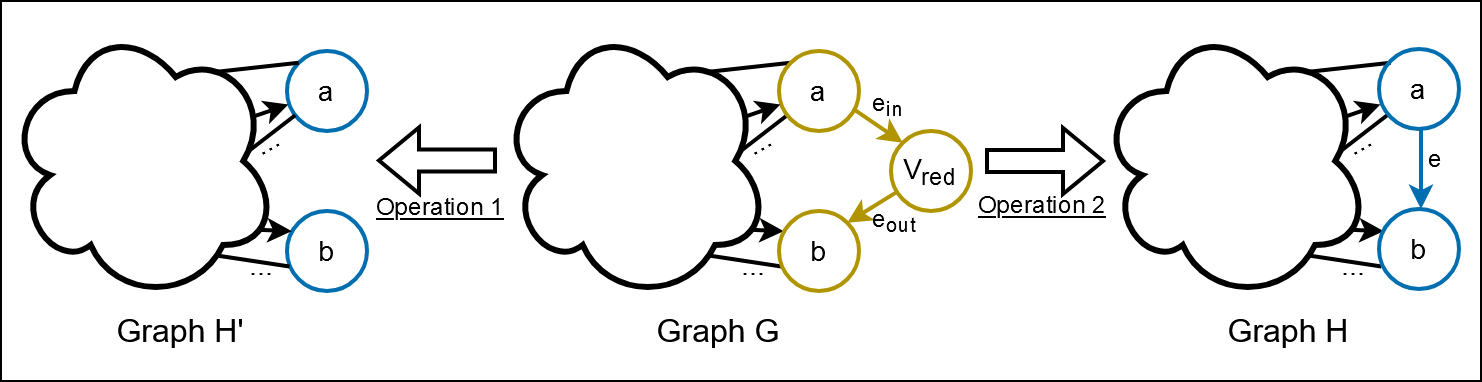
\includegraphics[width=\textwidth]{fig4_b.png}
    \caption{Demonstration of Operation 1 and Operation 2 on a edge-critical strongly connected digraph $\mathcal{G}$ resulting into digraphs $\mathcal{H'}$ and $\mathcal{H}$ respectively. Either $\mathcal{H'}$ or $\mathcal{H}$ is also edge-critical strongly connected digraph.}
    \label{fig:fig4}
\end{figure}

\noindent We shall now prove the most important theorem regarding edge-critical strongly connected digraphs.

\subsection{Completeness of the Construction Algorithm}

\begin{theorem}
Any edge-critical strongly connected digraph must contain a node with degree 2.
% i.e. only one in-edge ($e_{in}$) and only one out-edge ($e_{out}$)
\end{theorem}

\begin{proof}
We prove the theorem by assuming there exist an edge-critical strongly connected digraph ($\mathcal{G}$) of N nodes, such that all its node have degree 3 or more and showing that the assumption leads to a contradiction. To do so, select any arbitrary node A of the graph $\mathcal{G}$ and construct a spanning tree rooted at the node A. ...Complete the rules for construction of spanning tree here...

\vspace{0.5em} % Adds a small vertical gap
\noindent Now, one of the following three scenarios must be true for any leaf of the spanning tree:
\begin{enumerate}
    \item The leaf has two or more out-edges only.
    \item The leaf has two or more in-edges only.
    \item The leaf has one in-edge and one or more out-edges.
\end{enumerate}

\subsubsection{Scenario 1: A leaf has two or more out-edges only} This is clearly not possible as the leaf node would then have out-edges only and no in-edge. Thus, it is not possible to reach from any node on the graph $\mathcal{G}$ to this node.

\subsubsection{Scenario 2: A leaf has two or more in-edges only} We deconstruct this case using the following logic to show that it is not possible to have two or more in-edges only on any leaf.

\subsubsection{Scenario 3: A leaf has one in-edge and two or more out-edges} We deconstruct this case too using the following logic to show that it is not possible.

\subsubsection{Conclusion} We have shown that all of the possible scenarios for a leaf on the constructed spanning tree is infeasible. Thus, our assumption that there exists an edge-critical strongly connected digraph ($\mathcal{G}$) of N nodes, such that all its nodes have degree 3 or more is incorrect.
\end{proof}


\begin{credits}
\subsubsection{\ackname} A bold run-in heading in small font size at the end of the paper is
used for general acknowledgments, for example: This study was funded
by X (grant number Y).

\subsubsection{\discintname}
It is now necessary to declare any competing interests or to specifically
state that the authors have no competing interests. Please place the
statement with a bold run-in heading in small font size beneath the
(optional) acknowledgments\footnote{If EquinOCS, our proceedings submission
system, is used, then the disclaimer can be provided directly in the system.},
for example: The authors have no competing interests to declare that are
relevant to the content of this article. Or: Author A has received research
grants from Company W. Author B has received a speaker honorarium from
Company X and owns stock in Company Y. Author C is a member of committee Z.
\end{credits}
%
% ---- Bibliography ----
%
% BibTeX users should specify bibliography style 'splncs04'.
% References will then be sorted and formatted in the correct style.
%
% \bibliographystyle{splncs04}
% \bibliography{mybibliography}
%
\begin{thebibliography}{8}
\bibitem{ref_article1}
Author, F.: Article title. Journal \textbf{2}(5), 99--110 (2016)

\bibitem{ref_lncs1}
Author, F., Author, S.: Title of a proceedings paper. In: Editor,
F., Editor, S. (eds.) CONFERENCE 2016, LNCS, vol. 9999, pp. 1--13.
Springer, Heidelberg (2016). \doi{10.10007/1234567890}

\bibitem{ref_book1}
Author, F., Author, S., Author, T.: Book title. 2nd edn. Publisher,
Location (1999)

\bibitem{ref_proc1}
Author, A.-B.: Contribution title. In: 9th International Proceedings
on Proceedings, pp. 1--2. Publisher, Location (2010)

\bibitem{ref_url1}
LNCS Homepage, \url{http://www.springer.com/lncs}, last accessed 2023/10/25
\end{thebibliography}
\end{document}
